% Defino el tipo de documento.
\documentclass[a4paper,11pt]{article}

% Este paquete permite hacer encabezados y pies de p�gina como
% Los de las gu�as de D�az.
%\usepackage{fancyhdr}

% Este es para poder poner gr�ficos y diagramas.
\usepackage{graphicx}

% Este paquete est� por las dudas... Si algun archivo eps se vuelve
% rebelde y no sale donde uno quiere, hay que encajarle "\FloatBarrier" antes
% y despues y listo.
\usepackage{placeins}



% Toda la configuraci�n del documento.
%\input{preambulo.tex}


%\usepackage{grffile}
%\usepackage[dvips]{graphicx}


\hyphenation{}

\renewcommand{\sectionmark}[1]{\markboth{}{\thesection\ \ #1}}


\title{Evaluaci\'on Final de Simulaci\'on de Sistemas }

\author{45.288 Brasca, Juan Alejandro\\45.020 Stancato, Lucila\\45.002 Modernell, Dami\'an\\45.418 Negro, Conrado Luis}
\date{}

% Empieza el documento.
\begin{document}
\maketitle



\section*{a)   Modelar el intervalo de tiempo entre arribos, a partir de los datos medidos del archivo
llegadasregistro y modelar el intervalo de tiempo de atenci\'on de la estaci\'on E3 con los
datos del archivo e3registro. Para ello hacer estad\'istica descriptiva, justificando el n\'umero
de intervalo de clases y realizar los test pertinentes.
}

\subsection*{Tiempo entre arribos al sistema}
Mediante mediciones del horario de arribo de clientes al sistema, computamos
los intervalos de tiempo entre arribos, y los representamos en el histograma
de la figura 1. Est\'a dividido en 7 intervalos de clase determinados a partir
de la f\'ormula de Sturgess que observamos en la ecuaci\'on 1.1.
\begin{equation}
 k = 1 + 3.3  Log(n)  \hspace{6cm} 
\end{equation}
donde $k$ es el N$^o$ de intervalos y $n$ es el N$^o$ de muestras.

\begin{figure}
\begin{center}
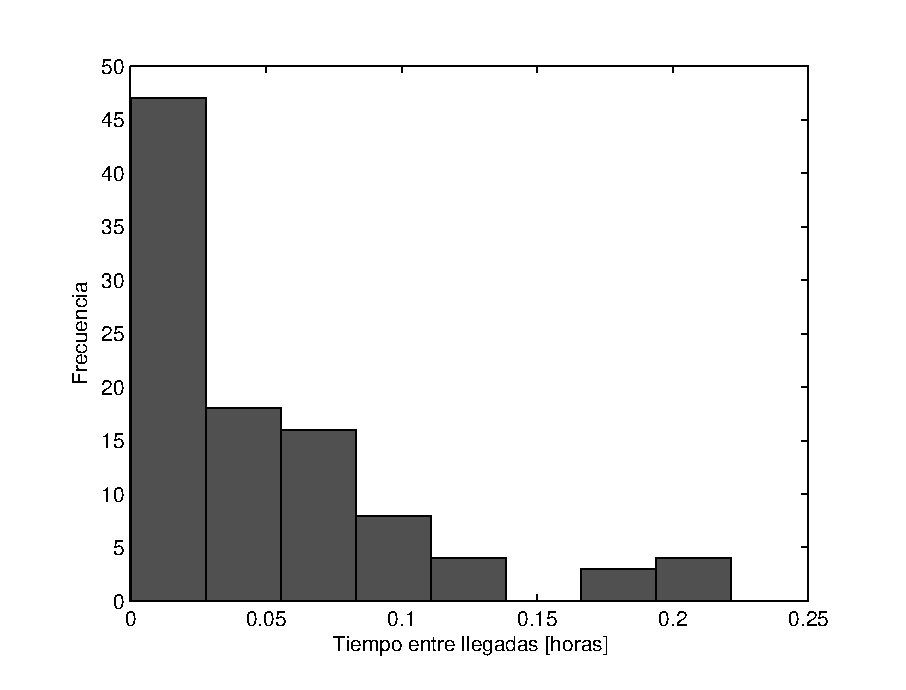
\includegraphics[width=11cm]{histograma_llegadas}
\caption{Histograma de intervalos de tiempo entre arribos de clientes al sistema. Se puede observar que parece provenir de una variable aleatoria con distribuci\'on exponencial.}
\end{center}
\end{figure}

Para determinar si la distribuc\'on de probabilidad del tiempo entre arribos
de clientes al sistema es exponencial, realizamos el test de bondad de ajuste
$\chi^2$. Las hip\'otesis del test son:

\begin{itemize}
 \item {$H_{0}$:} $\chi_{0}^2 < \chi_{n-1,\alpha}$ (Las llegadas de clientes al sistema est\'an exponencialmente distribuidas)
 \item {$H_{1}$:} $\chi_{0}^2 \ge \chi_{n-1,\alpha}$ (Las llegadas de clientes al sistema NO est\'an exponencialmente distribuidas)
\end{itemize}

A partir de las mediciones y de los valores esperados para cada
intervalo de clase, computamos el estad\'istico $\chi_{0}^2 = 10.709$. Como el valor
cr\'itico con un nivel de significaci\'on de 5\% y con 5 grados de libertad resulta 
$\chi_{0.05,5}^2 = 11.07$, rechazamos $H_1$ en favor de $H_0$.\\
Tambi\'en realizamos el test de Kolmogorov-Smirnov sobre las mediciones de los tiempos de arribos, agrupadas en los intervalos 
de clase que mencionamos previamente. Obtenemos el estad\'istico para dichos datos $D =  0,1238$, con un valor cr\'itico para un nivel
de significaci\'on $\alpha = 0.05 \% $, que es  $D_{7,\alpha} = 0.4834$. Luego al ser $D < D_{t, \alpha }$, podemos conclu\'irir que se pasa el test.
Finalmente podemos suponer, habiendo pasado ambos tests, que los arribos de clientes al sistema estan distribuidos exponencialmente, con una tasa media de 18.825.

\subsubsection*{Tasa de servicio de la estaci\'on $E3$}
Analizamos los tiempos de servicio de la estaci\'on $E3$ medidos del sistema, y volcamos
los datos a un histograma (ver figura 2) de 8 intervalos de clase tambi\'en computados
a partir de la f\'ormula de Sturgess.

\begin{figure}
\begin{center}
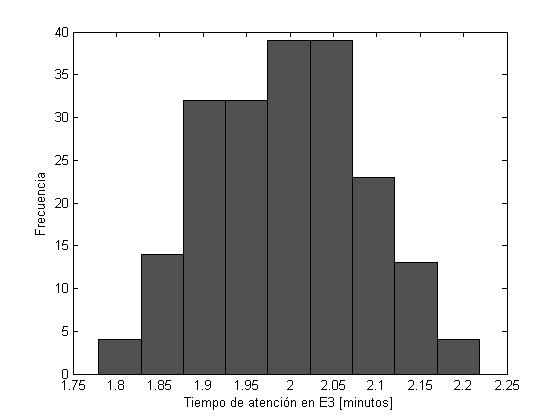
\includegraphics[width=11cm]{histograma_e3}
\caption{Histograma de la medici\'on de los tiempos de servicio del servidor $E3$. Observamos que los datos parecen provenir de una variable aleatoria con distribuci\'on normal.}
\end{center}
\end{figure}

En la figura 2, observamos que los datos parecen provenir de una variable aleatoria con distribuci\'on normal.
Para poder determinar si esto es cierto, realizamos el test estad\'istico $\chi^2$ con las siguientes hip\'otesis:

\begin{itemize}
 \item {$H_{0}$:} $\chi_{0}^2 < \chi_{n-1,\alpha}$ (El tiempo de servicio de la estaci\'on $E3$ es una variable aleatoria con distribuci\'on normal)
 \item {$H_{1}$:} $\chi_{0}^2 \ge \chi_{n-1,\alpha}$ (El tiempo de servicio de la estaci\'on $E3$ NO es una variable aleatoria con distribuci\'on normal)
\end{itemize}

Estimamos la media y la varianza de la distribuci\'on resultando:
\begin{itemize}
 \item {$\mu$ =} $1.995$
 \item {$\sigma^2$ =}  $0.008332$
\end{itemize}

El valor del estad\'istico resulta $\chi_{0}^2 = 4,7492$, y como el valor
cr\'itico es $\chi_{5,0.05}^2 = 11.07$ rechazamos $H_1$ en favor de $H_0$.

\section*{b) Indicar las variables de estado del sistema y el espacio de estado.}

\begin{figure}
\begin{center}
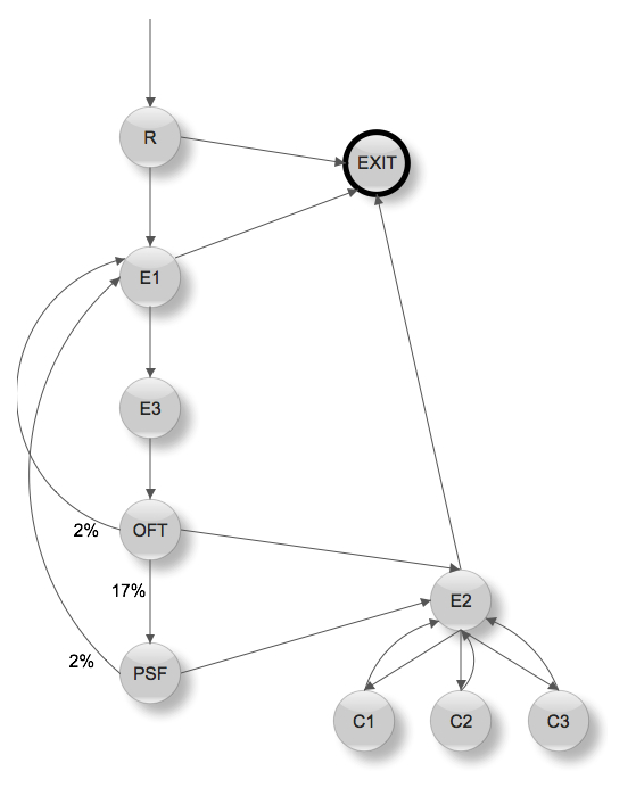
\includegraphics[width=6cm]{automata}

\caption{Modelo del sistema de renovaci\'on del registro}
	\end{center}
\end{figure}

Considerando el gr\'afico de la figura 3,  definimos el espacio de estados\\

$ S = \{ ( x_R, x_{E_1}, x_{OFT}, x_ {PSF}, x_{E_2}, x_{E_3}, x_{C_1}, x_{C_2}, x_{C_3},$ \\
    $y_R, y_{E_1}, y_{OFT}, y_ {PSF}, y_{E_2}, y_{E_3}, y_{C_1}, y_{C_2}, y_{C_3} ) \/ $ \\
     $x_R, x_{E_1}, x_{OFT}, x_ {PSF}, x_{E_2}, x_{E_3}, x_{C_1}, x_{C_2}, x_{C_3} = 1, 2, 3, ...$\\
     $\wedge y_R, y_{E_1}, y_{OFT}, y_ {PSF}, y_{E_2}, y_{E_3}, y_{C_1}, y_{C_2}, y_{C_3} =  0, 1 \}$


Donde: \\
 $x_R$ es la longitud de la cola de recepci\'on.\\
$x_{E_1}$ es la longitud de la cola del servidor E1.\\
$x_{E_2}$ es la longitud del servidor E2.\\
$x_{E_3}$ es la longitud del servidor E3.\\
$ x_{OFT}$ es la longitud de la cola de oftalmolog\'ia.\\
$x_ {PSF}$ es la longitud de la cola del estudio Psico-F\'isico.\\
$x_{C_1}$ es la longitud de la cola de la caja C1.\\
$x_{C_2}$es la longitud de la cola de la caja C2.\\
$x_{C_3}$es la longitud de la cola de la caja C3.\\ \\
\noindent
$y_R$ Ocupac\'on de la recepci\'on.\\
$y_{E_1}$ Ocupaci\'on de la estaci\'on E1.\\
$y_{E_2}$ Ocupaci\'on de la  estaci\'on E2.\\
$y_{E_3}$ Ocupaci\'on de la  estaci\'on E3.\\
$ y_{OFT}$ Ocupaci\'on de la oficina de oftalmolog\'ia\\
$y_ {PSF}$ Ocupaci\'on de la oficina Psico-Fisica.\\
$y_{C_1}$ Ocupaci\'on de la caja 1.\\
$y_{C_2}$ Ocupaci\'on de la caja 2.\\
$y_{C_3}$ Ocupaci\'on de la caja 3.\\

\section*{c) Indicar los tipos de eventos y el espacio de eventos.}
El espacio de eventos del sistema lo definimos como:\\

$E = \{ A, D, r_{e1}, e1_{e3}, e3_{oft}, oft_{psf}, oft_{e2}, psf_{e2}, oft_{e1}, psf_{e1}, e2_{c1}, e2_{c2}, e2_{c3},  c1_{e2},
c2_{e2}, c3_{e3} \}$


Donde:\\
$A$ es la entrada de una persona a $R$.\\
$D$ es la partida de una persona del sistema. \\
$r_{e1}$ es la partida de una persona desde $R$ hacia  $E_1$\\
$e1_{e3}$ es la partida de una parsona de $E_1$ hacia $E_3$ \\
$e3_{oft}$ es la partida de una persona de $E_3$ hacia $OFT$\\
$oft_{psf}$ es la partida de una persona de $OFT$ hacia $PSF$.\\
$oft_{e2}$, $psf_{e2}$ son las partidas de una persona desde $OFT$ o desde $PSF$ hacia $E_2$.\\
$oft_{e1}$, $psf_{e1}$ son las partidas desde $OFT$ o de $PSF$ hacia $E_1$\\
$e2_{c1}$, $e2_{c2}$ y $e2_{c3}$ son las partidas desde $E_2$ hacia $C_1$, $C_2$ y $C_3$.\\ 
$c1_{e2}$, $c2_{e2}$ y $c3_{e2}$ son las partidas desde $C_1$, $C_2$ y $C_3$ hacia $E_2$.\\






\section*{d)      Realizar una simulaci\'on indicando las condiciones iniciales, el tipo de generador usado y
la semilla. Mostrar las g\'aficas de las colas en cada estaci\'on.
}

Para generar n\'umeros pseudoaleatorios, usamos el generador de L'Ecuyer con semillas 50 y 23 (recordando
que lo importante es que las semillas no sean cero).  El generador de L'Ecuyer genera una secuencia de n\'umeros
pseudoaleatorios con distribuci\'on uniforme entre 0 y 1.  A partir de esa secuencia, generamos secuencias de n\'umeros pseudoaleatorios
con distribuci\'on exponencial. Para generar una secuencia de n\'umeros pseudoaleatorios con distribuci\'on normal usamos
el generador de Box-Muller (usando el generador de L'Ecuyer para generar la secuencia que tiene distribuci\'on uniforme).

Para hacer la simulaci\'on consideramos que el porcentaje de personas con m\'as de 70 a\~nos es de 7\%.   Esto hace
que la probabilidad de que un cliente haga el examen de aptitud psico�f\'isica pase de un 10\% a un 17\%.  Consideramos tambi\'en
que un 20\% de los clientes vienen solamente a buscar el instructivo para hacer el tr\'amite y se van, y solamente el 80\% hace el tr\'amite.
Adem\'as suponemos que un cliente tarda entre 0.5 y 2 minutos en llenar el formulario que le entregan en la estaci\'on $E1$, 
y lo simulamos con una variable pseudo-aleatoria uniformemente distribuida.
Para las cajas $C_1$, $C_2$ y $C_3$, asumimos que los clientes se encolan en la caja que tenga menos personas, siempre optando primero por
$C_1$, luego por $C_2$ y como \'ultima opci\'on por $C_3$.  

Con estas consideraciones, realizamos una simulaci\'on que termina a las 16:56 hs y atiende a 128 clientes.







\section*{e)     Realizar 10 simulaciones independientes. Hallar el tiempo medio por cliente en el sistema,
suponiendo que las tres cajas C1, C2 y C3 est\'an operativas mostrar los resultados convenien-
temente en una tabla. Computar con estos resulatados el estimador del tiempo medio por
cliente y su error.
}
\section*{f)    Si la probabilidad de que la caja C3 est\'e operativa es p, computar el tiempo medio por
cliente en el sistema en funci\'on de p. Graficar.
}
\section*{g)   Computar la probabilidad de que el tiempo medio de espera en la cola de OFT sea mayor
a 5 minutos
}

La variable aleatoria $OFT$ tiene distribuci\'on exponencial con tiempo medio de 3.5 minutos. Para determinar la probabilidad de que el tiempo medio
de espera sea mayor a 5 minutos la obtenemos a trav\'es de las ecuaciones XXXXXXXXXXX

\begin{equation}
 P( OFT > 5 ) = 1 - P( OFT \leq 5 )
\end{equation}
entonces:
\begin{equation}
P(OFT > 5 ) = 1 - ( 1 - e^{- \frac{1}{3.5}5} )
\end{equation}
Finalmente la probabilidad resulta:
\begin{equation}
 P( OFT > 5 ) = 0.2397
\end{equation}


\begin{thebibliography}{1}
\bibitem{IEEhowto:kopka}
http://es.wikipedia.org/wiki/Regla\_de\_Sturgess
\end{thebibliography}


\end{document}
